% ---------------------------------------------------------------------------
% ShortageGraph  --  IEEE EMBC 2027 submission draft
%
% FORMAT RULES (embc.embs.org/2027/author-guidelines, checked 2026-10-28):
%   * Pages 1-4: technical text, figures, tables, equations.
%   * Page 5: acknowledgments and references ONLY (enforced with \clearpage).
%   * Maximum 20 references.
%   * Stock IEEEtran[conference] -- no margin, font or column changes.
%
% WHAT THIS VERSION IS
%   The retrospective forecasting design cannot be trained: its labels cannot be
%   certified (Section IV and shortagegraph/labels.py). The paper therefore
%   reports (a) a cross-sectional study whose exposures and outcome all come
%   from data that exist, (b) the audit explaining what the public record cannot
%   support, and (c) the specification of the forecasting system those labels
%   were meant to train -- restored from the original design, implemented in
%   this repository, and reported without any performance number.
%   Every number below is produced by code in this repository:
%     python -m shortagegraph.realdata      -> Table I (network)
%     python -m shortagegraph.casecontrol   -> Table II/III (associations)
%     python -m shortagegraph.labels --audit-> Section IV (coverage audit)
%
% BEFORE SUBMITTING: fill the author block, funding, AI disclosure and URL.
%
% COMPILE: tectonic main.tex      (or IEEEtran in Overleaf)
% ---------------------------------------------------------------------------
\documentclass[conference,letterpaper]{IEEEtran}

\usepackage{cite}
\usepackage{amsmath,amssymb}
\usepackage{graphicx}
\usepackage{booktabs}
\usepackage{xcolor}
\usepackage{tikz}
\usetikzlibrary{arrows.meta,positioning}
\usepackage{url}

% Unfilled-number marker: renders red so nothing slips through unnoticed.
\newcommand{\ph}[1]{\textcolor{red}{#1}}

\begin{document}

\title{ShortageGraph: Recall Exposure and Market Structure in the U.S. Drug\\
Shortage Snapshot, and the Limits of Public Onset Labels}

\author{\IEEEauthorblockN{Ananya Sukruta Mysore\IEEEauthorrefmark{1} and
Avani Agarwal\IEEEauthorrefmark{2}}
\IEEEauthorblockA{\IEEEauthorrefmark{1}\ph{Department, Institution, City,
State ZIP, USA}\\\ph{email}}
\IEEEauthorblockA{\IEEEauthorrefmark{2}\ph{Department, Institution, City,
State ZIP, USA}\\\ph{email}}}

\maketitle

\begin{abstract}
Hospital pharmacists usually learn of a drug shortage only after it is posted,
so predicting which drugs will be listed next is an attractive target for
clinical informatics. Published models are tabular and supervised on historical
posting labels, which presumes that history is complete. We test that
presumption and then ask what the public record can support instead. First, we
build the U.S. drug supply network from the National Drug Code directory:
10{,}537 drug nodes with 88{,}071 edges at the median week, of which 68.0\% have
a single labeler. Second, we conduct a cross-sectional study at a single
reference date (22 October 2026), comparing 293 drugs on the FDA shortage list
with 14{,}313 marketed drugs not on it. A recall of the same product in the
preceding 24 months was present for 17.1\% of listed drugs versus 2.5\% of
unlisted ones (odds ratio 8.07, 95\% CI 5.85--11.13); because cases are
ascertained through product codes, we re-estimate within product-count strata,
where the pooled odds ratio falls to 3.64 and four of five strata still exclude
unity. The association holds for injectables (14.1\% versus 3.7\%, odds ratio
4.29). Finally, we show that the openFDA shortage mirror holds 1{,}142 current
entries but only 19 resolved ones, so first-posting labels are
survivorship-biased; a released gate refuses to train on uncertified years.
Finally, we specify the forecasting system those labels were meant to train
---relational message passing, a monotone hazard head, occlusion attribution and
a 25-drug weekly review list---and report no performance for it, because a
number computed on those labels would describe the bias. Code for all of it is
released.
\end{abstract}

\begin{IEEEkeywords}
drug shortages, supply network, cross-sectional study, graph neural networks,
reproducibility
\end{IEEEkeywords}

\section{Introduction}

Drug shortages are a persistent threat to patient care, with well documented
clinical cost: delayed and cancelled therapy, medication errors and forced
switches to less familiar agents \cite{mclaughlin}. The American Society of
Health-System Pharmacists counted 227 active national shortages at the end of the
second quarter of 2026, down from 323 in early 2024 but rising for consecutive
quarters, and just under half of new shortages involved single-manufacturer
products \cite{ashp}. The FDA attributes most shortages to manufacturing and
quality problems concentrated in few facilities \cite{fdataskforce}, which makes
the supply network, not any single drug, the natural unit of analysis.

Prediction work in this area is young. Pall \emph{et al.} \cite{pall} built
supervised models from the sales records of 22 Canadian pharmacies; Roe
\emph{et al.} \cite{roe} modelled duration and cause from 1{,}054 Korean
reports. Both treat each drug as an independent row. Eberhardt \emph{et
al.} \cite{eberhardt} constructed a descriptive knowledge graph of the German
supply chain to find critical suppliers, and Kosasih \emph{et al.} \cite{kosasih}
applied graph neural networks to supply chain risk, but neither forecasts
shortages. All supervised approaches share one dependency: a trustworthy
historical label of when each drug entered shortage.

That dependency would be worth the trouble because shortage risk is relational:
a quality event at one facility threatens every product made there, and a drug
with few labelers is exposed through each of them. Those two-hop paths carry
signal that a row of per-drug counts cannot represent.

This paper started as an attempt to build that label for the United States and
ended by testing it. Our contributions are:
\begin{enumerate}
\item \emph{A measured network.} A weekly-dated graph of U.S. drug products and
the labelers that market them, reconstructed from the National Drug Code
directory \cite{ndc} over 96 sampled weeks, with the concentration statistics
that motivate relational analysis (Table~\ref{tab:network}).
\item \emph{A cross-sectional association study.} At one reference date, drugs
on the FDA shortage list are compared with all other marketed drugs on two
exposures that need no shortage history: whether the same product was recalled
recently, and how many labelers market it (Tables~\ref{tab:assoc}
and~\ref{tab:strata}).
\item \emph{A label-provenance audit.} We quantify why the openFDA shortage
record cannot support first-onset forecasting, and release a gate that refuses
to train on years it cannot certify,   so the failure is caught rather than
silently learned.
\item \emph{A released system, and no claim about it.} The relational model,
monotone hazard head, attribution rule and evaluation harness are specified,
implemented and unit-tested (Section~\ref{sec:system}), with no test performance
reported, for the reason Section~\ref{sec:audit} establishes.
\end{enumerate}

\emph{Clinical relevance}---A recall of the same product is the kind of signal a
pharmacy already receives, weeks or months before a shortage appears on a
national list. Knowing that this signal is enriched among listed drugs, and by
how much, tells a procurement pharmacist where to look first, and tells the
informatics community which labels are safe to learn from.

\section{Data and Study Design}

\subsection{Supply Network from the NDC Directory}
Every marketed U.S. drug product carries a National Drug Code. We parse the
directory \cite{ndc} into 114{,}018 products and aggregate them into drug nodes
keyed by active ingredient set, dosage form and route, which matches the unit in
which FDA shortage entries are reported. A product is active at a date if its
marketing start has passed and its marketing end has not. Two relations are
built per snapshot: \emph{markets} (drug--labeler) and \emph{substitutes}
(drug--drug, same ingredients with a different form or route).

Manufacturing establishments are deliberately absent: linking products to FDA
Establishment Identifiers requires the NDC-to-FEI mapping from DailyMed
Structured Product Labeling \cite{dailymed}, which this study does not claim to
have completed. Counts reported here describe product and labeler structure
only, and no result uses two-hop facility paths.

\begin{table}[t]
\caption{Measured network structure. Values are medians over 96 monthly
snapshots, 2018--2025, computed from 114{,}018 NDC products.}
\label{tab:network}
\centering
\footnotesize
\begin{tabular}{@{}lr@{}}
\hline
Quantity & Value\\
\hline
Sampled weekly snapshots & 96\\
Drug nodes $|V_D|$ & 10{,}537\\
Labeler nodes $|V_L|$ & 4{,}391\\
Edges (markets $+$ substitutes) & 88{,}071\\
Drugs with a single labeler & 68.0\%\\
Median labelers, drugs on shortage list & 4\\
Median labelers, drugs not on list & 1\\
\hline
\end{tabular}
\end{table}

\subsection{Reference Date, Cases and Controls}
The shortage records come from the openFDA shortage endpoint \cite{openfda},
which mirrors the FDA Drug Shortages Database \cite{fdads}. We take the latest
\emph{initial posting date} present, 22 October 2026, as the single reference
date; using one date for every subject is what makes the design interpretable,
because exposure windows then have a common end.

A drug is a \emph{case} if any shortage record maps into the network at the
reference date (current or to-be-discontinued status), and a \emph{control} if
it is active in the directory then and never appears in the shortage records. Of
1{,}604 records, 1{,}279 (79.7\%) carry an NDC that resolves to a study drug,
yielding 293 distinct case drugs; 325 (20.3\%) could not be mapped and are
excluded, and controls number 14{,}313. This is a prevalence case-control study,
reported as a cross-sectional association; it estimates neither incidence nor
causal effect. Fig.~\ref{fig:design} shows how the groups are assembled, and the
asymmetry in how they are found is why Table~\ref{tab:strata} exists.

\begin{figure}[t]
\centering
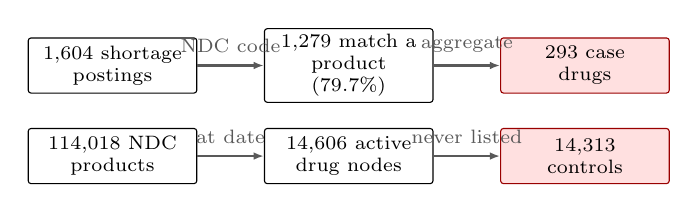
\begin{tikzpicture}[font=\scriptsize,
  bx/.style={draw, rounded corners=1pt, align=center, inner sep=2pt,
    minimum height=7mm, text width=20mm},
  hl/.style={bx, fill=red!12, draw=red!60!black},
  arr/.style={-{Latex[length=1.3mm]}, thick, black!65}]
\node[bx] (p) at (0,1.15) {1{,}604 shortage\\postings};
\node[bx] (m) at (3.0,1.15) {1{,}279 match a\\product (79.7\%)};
\node[hl] (c) at (6.0,1.15) {293 case\\drugs};
\node[bx] (n) at (0,0) {114{,}018 NDC\\products};
\node[bx] (u) at (3.0,0) {14{,}606 active\\drug nodes};
\node[hl] (k) at (6.0,0) {14{,}313\\controls};
\draw[arr] (p) -- (m);
\draw[arr] (m) -- (c);
\draw[arr] (n) -- (u);
\draw[arr] (u) -- (k);
\node[above=0.4mm, font=\scriptsize, black!65] at (1.5,1.15) {NDC code};
\node[above=0.4mm, font=\scriptsize, black!65] at (4.5,1.15) {aggregate};
\node[above=0.4mm, font=\scriptsize, black!65] at (1.5,0) {at date};
\node[above=0.4mm, font=\scriptsize, black!65] at (4.5,0) {never listed};
\end{tikzpicture}
\caption{How cases and controls are assembled at the reference date. A case
enters only when a posting carries an NDC that resolves to a marketed product,
so a drug with many listed products is easier to capture and easier to mark
exposed. That advantage is what the product-count stratification in
Table~\ref{tab:strata} controls.}
\label{fig:design}
\end{figure}

\subsection{Exposures}
Two exposure definitions are used, and they are kept separate because they
differ in specificity.

\emph{Same-product recall.} An enforcement report \cite{openfda} published in
the 24 months before the reference date lists an NDC belonging to the drug node:
precise, because it identifies a recall of that product.

\emph{Any-labeler recall.} An enforcement report in the same window names a firm
that markets the drug --- broad, and, as Section~\ref{sec:disc} notes, partly a
measure of firm size.

\emph{Concentration.} The number of distinct labelers behind a drug, from the
directory alone.

Of 1{,}587 enforcement reports in the window, 808 carry an NDC that resolves to
a study drug. Because cases and exposures are both reached through NDC codes, a
drug with many products is easier to capture and easier to mark exposed, so we
treat product count as an ascertainment variable and stratify on it
(Section~\ref{sec:analysis}); this is the study's most important correction.

\subsection{Statistics}\label{sec:analysis}
Associations are reported as odds ratios with Katz 95\% confidence intervals and
two-sided Fisher exact tests, computed from the hypergeometric distribution
without approximation \cite{rothman}. Results are pooled across strata with the
Mantel--Haenszel estimator. Strata are defined two ways: by concentration
(single versus multiple labelers) and by product count (1, 2--3, 4--7, 8--20,
21 or more NDCs). The second is the ascertainment control; the first tests
whether concentration explains the recall association. Sensitivity analyses
repeat the exposure with 12- and 36-month windows. All computations are in
\texttt{shortagegraph.casecontrol}, which reports the 2$\times$2 table behind
every estimate.

\section{Results}

\begin{table}[t]
\caption{Cross-sectional associations at 22 October 2026 (293 cases, 14{,}313
controls; 24-month exposure window). OR: odds ratio; CI: Katz 95\% confidence
interval; $p$: two-sided Fisher exact.}
\label{tab:assoc}
\centering
\footnotesize
\setlength{\tabcolsep}{1.6pt}
\begin{tabular}{@{}lrrrrr@{}}
\hline
Exposure & Cases & Controls & OR & 95\% CI & $p$\\
\hline
Same-product recall & 17.1\% & 2.5\% & 8.07 & 5.85--11.13 & $1.7\!\times\!10^{-25}$\\
Any-labeler recall & 84.6\% & 22.9\% & 18.55 & 13.47--25.55 & $2.0\!\times\!10^{-107}$\\
Either definition & 85.3\% & 23.3\% & 19.18 & 13.85--26.57 & $2.2\!\times\!10^{-108}$\\
Single labeler & 22.5\% & 67.8\% & 0.14 & 0.11--0.18 & $1.1\!\times\!10^{-54}$\\
\hline
\end{tabular}
\end{table}

Table~\ref{tab:assoc} reports the crude associations. A recall of the same
product in the preceding 24 months is present for 17.1\% of listed drugs against
2.5\% of unlisted ones (OR 8.07, 95\% CI 5.85--11.13), and the broad firm-level
definition for 84.6\% against 22.9\% (OR 18.55). At 12 and 36 months the
same-product odds ratio is 8.97 and 8.31, so the finding does not depend on the
window.

\subsection{Ascertainment and the Concentration Result}
The crude concentration estimate points the other way from the premise that
motivates most shortage work: listed drugs are \emph{less} often single-labeler
(22.5\% versus 67.8\%, OR 0.14), with a median of four labelers against one. We
do not read this as evidence that competition protects supply: cases are found by
matching product codes, so a drug with many products is more likely to be
captured, and the same mechanism inflates any NDC-based exposure. It is therefore
reported as an ascertainment artefact, not a clinical finding.

The correction matters quantitatively. Within product-count strata the pooled
Mantel--Haenszel odds ratio falls from 8.07 to 3.64, so roughly half of the crude
association was the capture advantage of large products. Four of five strata
still exclude unity, including the 21-or-more stratum (OR 2.53, 95\% CI
1.45--4.42): attenuated, not removed.

\begin{table}[t]
\caption{Same-product recall, stratified by number of NDC products per drug
(ascertainment control). Pooled Mantel--Haenszel OR 3.64.}
\label{tab:strata}
\centering
\footnotesize
\setlength{\tabcolsep}{1.6pt}
\begin{tabular}{@{}lrrrrr@{}}
\hline
NDC products & Cases & Controls & OR & 95\% CI & $p$\\
\hline
1 & 34 & 7{,}581 & 29.60 & 9.89--88.59 & $2.2\!\times\!10^{-5}$\\
2--3 & 60 & 2{,}671 & 8.07 & 3.47--18.77 & $8.3\!\times\!10^{-5}$\\
4--7 & 48 & 1{,}470 & 2.38 & 0.83--6.87 & 0.107\\
8--20 & 87 & 1{,}618 & 4.17 & 2.29--7.61 & $3.3\!\times\!10^{-5}$\\
21+ & 64 & 973 & 2.53 & 1.45--4.42 & 0.002\\
\hline
\end{tabular}
\end{table}

\subsection{Concentration Does Not Explain the Signal}
Stratifying the recall association by concentration gives odds ratios of 14.06
(95\% CI 8.61--22.96) among single-labeler drugs and 13.11 (7.47--23.01) among
multi-labeler drugs, so the signal survives that stratification; only the
product-count stratification attenuates it, and only partially.

\subsection{Injectable Subgroup}
Injectables are the class whose absence most disrupts acute and oncology care.
Among 156 injectable case and 2{,}224 control drugs a same-product recall is
present for 14.1\% against 3.7\% (OR 4.29, 95\% CI 2.60--7.08), and the broad
definition for 87.2\% against 32.9\%. so the association holds where a procurement response is feasible.

\section{What the Public Record Cannot Support}\label{sec:audit}

The study above was designed after the forecasting design failed, and the reason
belongs in the record. First-posting labels require a complete history: a drug
missing from it looks never-listed, which turns an existing shortage into a false
negative rather than merely removing it.

The openFDA shortage mirror is a live snapshot, not an archive. Of 1{,}604
records, 1{,}142 are current, 443 are to be discontinued and only 19 are
resolved. A shortage that began in 2019 and resolved in 2021 is simply absent.
Collapsing to distinct drugs leaves 307, and per-year first-posting counts over
the intended training window are 13 (2018), 4 (2019), 17 (2020), 11 (2021) and
18 (2022), against the hundreds the FDA recorded annually.

We did not attempt to repair this by modelling. Instead,
\texttt{shortagegraph.labels} computes coverage per year, checks that postings
match the network's keys, and refuses to certify a window below a stated floor;
\texttt{train.py} exits rather than training on an uncertified window. Both
splits fail certification, and the released code reproduces that failure. The
obvious escape routes are closed: the Wayback Machine has no usable snapshots of
the legacy shortage listing page, and the FDA Data Dashboard returns HTTP 403 to
automated clients. A complete history would have to come from an FDA archival
export, a commercial shortage dataset, or a partner health system's own records.

\section{The System These Labels Would Train}\label{sec:system}

The audit above says which labels are unavailable; this section specifies what
would be fitted to them. Most of the specification does not depend on the
labels, and every component named here exists in the released code and is
covered by the test suite.

\subsection{Graph and Dated Features}
A snapshot at week $t$ is a heterogeneous graph
$G_t=(V_D\cup V_L,\{E_r\}_{r\in R},X_t)$ with drug nodes $V_D$ and labeler
nodes $V_L$. Two relations are built: \emph{markets} (drug--labeler) and
\emph{substitutes} (drug--drug, same ingredients, different form or route),
each with reverse edges so information flows both ways. Facility nodes are
absent, because the NDC-to-FEI mapping is not built, so with $K=2$ layers a
drug reaches its co-marketed products through a shared labeler. That is a
weaker version of the two-hop facility path the design was built around, and no
result here depends on it. All features come from records published on or
before $t$, over trailing windows of 13, 26 and 52 weeks, keyed to disclosure
dates rather than event dates so that no feature precedes publication; recalls
contribute counts by class and weeks since the most recent report.

\subsection{Monotone Hazard Head and Attribution}
For $h\in\{4,8,12\}$ weeks the label is
$y^{(h)}_{v,t}=\mathbf{1}[t<\tau_v\le t+h]$ with $\tau_v$ the week of first
posting, restricted to drugs never yet listed, and snapshots whose label
windows would cross a split boundary are embargoed --- a rule
\texttt{config.py} implements and the suite checks for leakage. Fitting three
independent classifiers can return a higher 4-week than 12-week risk, so we
model a discrete hazard over $(0,4]$, $(4,8]$ and $(8,12]$ instead,
\begin{equation}
\lambda_{v,j}=\sigma(w_j^\top h_v+b_j),\qquad
p^{(h_m)}_{v}=1-\prod_{j=1}^{m}\bigl(1-\lambda_{v,j}\bigr),
\end{equation}
which is monotone in $m$ by construction. The encoder is relational message
passing with mean aggregation\cite{rgcn,graphsage},
\begin{equation}
 h_v^{(k+1)}=\sigma\Bigl(W_0^{(k)}h_v^{(k)}
 +\sum_{r\in R}\sum_{u\in N_r(v)}\frac{1}{|N_r(v)|}W_r^{(k)}h_u^{(k)}\Bigr),
\end{equation}
trained on class-weighted cross-entropy with $\alpha=\sqrt{n_-/n_+}$, the square
root because the full ratio over-weighted the few positives in development. Baselines see the same drug-level features, with
labeler signals pre-aggregated as counts and maxima: a sole-source rule,
$L_2$ logistic regression, gradient-boosted trees\cite{xgboost} and an
edge-free MLP, the last isolating the value of structure from model capacity.
An alert is explained by occlusion,
$\Delta_{u\to v}=p(G_t)-p(G_t\setminus u)$, which replaces one upstream node's
features by their training median while leaving topology intact; occlusion is
preferred to a learned mask such as GNNExplainer\cite{gnnexplainer} because a
pharmacist can read it directly.

\subsection{Protocol, and Why Nothing Is Reported}\label{sec:status}
Positives are rare, so the primary metric is AUPRC\cite{saito}, with AUROC,
precision in a weekly 25-drug review list sized to pharmacy workload, the Brier
score, bootstrap intervals resampling drugs rather than drug-weeks, lead time
before posting, and an injectable subgroup. The harness implements each, and the
pipeline runs end to end on a synthetic fixture that verifies mechanics only:
shapes, label semantics, absence of future leakage, metric agreement with
reference implementations, and monotonicity of the hazard head. We report no test
performance, and the omission is the point.
Section~\ref{sec:audit} shows the label history is survivorship-biased, so a
model fitted to it would learn which shortages were recorded, not which drugs
failed; \texttt{train.py} refuses to fit on an uncertified history rather than
emitting such a number. 

\section{Discussion and Limitations}\label{sec:disc}

The central limitation is design: a single cross-section estimates who is in
shortage at one date, not who will be. It cannot show that a recall precedes an
onset, and for a drug listed for years a 2025 recall may follow the shortage
rather than lead it. Reverse causation is therefore compatible with our numbers,
and the finding is best read as co-occurrence, consistent with the FDA's
root-cause analysis \cite{fdataskforce} but not proof of it.

The broad exposure definition is nearly a measure of firm size, since a large
labeler has many recalls and many products; we report it for completeness and
rely on the same-product definition, which is narrow enough to mean something.

Case ascertainment is the other constraint: because cases are reached through
product codes, the concentration estimate and part of the recall estimate are
shaped by how many products a drug has, which the stratified analysis quantifies
rather than removes. A study with an independent case source, such as a health
system's shortage log, would not share the bias.

Public data also omit what determines supply --- ingredient sourcing, inventory,
contracts and demand surges --- so a public-data association is a floor, not a
ceiling. And the shortage list reflects reporting behaviour as much as scarcity,
so a study keyed to one list partly models that list.

The practical implication is nonetheless usable. A recall of the same product is
already known to a pharmacy when it happens, and it is enriched among drugs that
appear on the national shortage list. That supports using recall history to
prioritise which products a procurement pharmacist checks first, within existing
allocation rules, while the forecasting question waits for labels that can be
certified.

Two limits are specific to the system in Section~\ref{sec:system}. Deployment
carries a risk the design creates: if many institutions stockpile on one alert,
the forecast can cause the shortage it predicts, so a review list belongs inside
existing allocation rules and beside stewardship, not in a purchasing trigger.
And a retrospective design cannot show that earlier warning improves outcomes;
the step that could is a silent prospective evaluation, with alerts logged but
not acted on and scored against a partner's own shortage records.

\section{Conclusion}

We rebuilt the U.S. drug supply network from public listing data and asked what
it can support. Cross-sectionally, same-product recall exposure is strongly
associated with being on the shortage list (OR 8.07 crude, 3.64 after
stratifying on product count, 4.29 in injectables), while the sole-source premise
is not recoverable from list-based labels, because case ascertainment favours
large products. First-onset labels cannot be certified, so we release the gate
that says so rather than a model trained on corrupt negatives, plus the relational
model and protocol a certifiable source would train: the design survives its own
audit as a reproducible benchmark, not a withdrawn claim. Code is at
\url{https://github.com/ohtherewegoagain/shortagegraph}.

% References must begin on page 5: EMBC 2027 reserves pages 1-4 for technical
% content and page 5 for acknowledgments and references only.
\clearpage

\section*{Acknowledgment}

\emph{\ph{Funding sources, compute support and data-access acknowledgments.}}
Per EMBC 2027 AI-use policy, AI-generated content is disclosed here: the
manuscript text and analysis code were drafted with an AI coding assistant, and
the data figures were produced by the released code rather than drawn by hand.
\emph{\ph{Name the tool and confirm the sections covered.}}

\begin{thebibliography}{16}

\bibitem{ashp} American Society of Health-System Pharmacists and University of
Utah Drug Information Service, ``National drug shortages: January 2001 to June
2026,'' ASHP Drug Shortages Statistics, 2026. [Online]. Available:
https://www.ashp.org/drug-shortages/shortage-resources/drug-shortages-statistics

\bibitem{mclaughlin} M. McLaughlin, D. Kotis, K. Thomson \emph{et al.},
``Effects on patient care caused by drug shortages: a survey,'' \emph{J.
Manag. Care Pharm.}, vol. 19, no. 9, pp. 783--788, 2013.

\bibitem{fdataskforce} U.S. Food and Drug Administration, Drug Shortages Task
Force, ``Drug shortages: Root causes and potential solutions,'' FDA, Silver
Spring, MD, USA, 2019.

\bibitem{pall} R. Pall, Y. Gauthier, S. Auer, and W. Mowaswes, ``Predicting drug
shortages using pharmacy data and machine learning,'' \emph{Health Care Manag.
Sci.}, vol. 26, no. 3, pp. 395--411, 2023.

\bibitem{roe} H. S. Roe \emph{et al.}, ``Drug shortage in South Korea: machine
learning-based prediction models and analysis of duration and causal factors,''
\emph{Front. Pharmacol.}, vol. 16, art. 1608843, 2025.

\bibitem{eberhardt} K. Eberhardt, A. Schw\"arzel, F. K. Kaiser, S. Rosenberg,
and F. Schultmann, ``Leveraging knowledge graphs in pharmaceutical supply
chains: insights into key drivers of drug shortages,'' \emph{Int. J. Prod.
Res.}, vol. 63, no. 19, pp. 7129--7152, 2025.

\bibitem{kosasih} E. E. Kosasih, F. Margaroli, S. Gelli, A. Aziz, N. Wildgoose,
and A. Brintrup, ``Towards knowledge graph reasoning for supply chain risk
management using graph neural networks,'' \emph{Int. J. Prod. Res.}, vol. 62,
no. 15, pp. 5596--5612, 2024.

\bibitem{ndc} U.S. Food and Drug Administration, ``National Drug Code
Directory.'' [Online]. Available:
https://www.fda.gov/drugs/drug-approvals-and-databases/national-drug-code-directory

\bibitem{openfda} T. A. Kass-Hout \emph{et al.}, ``OpenFDA: an innovative
platform providing access to a wealth of FDA's publicly available data,''
\emph{J. Am. Med. Inform. Assoc.}, vol. 23, no. 3, pp. 596--600, 2016.

\bibitem{dailymed} U.S. National Library of Medicine, ``DailyMed.'' [Online].
Available: https://dailymed.nlm.nih.gov

\bibitem{fdads} U.S. Food and Drug Administration, ``FDA Drug Shortages
Database.'' [Online]. Available: https://dps.fda.gov/drugshortages

\bibitem{rothman} K. J. Rothman, S. Greenland, and T. L. Lash, \emph{Modern
Epidemiology}, 3rd ed. Philadelphia, PA, USA: Lippincott Williams \& Wilkins,
2008.

\bibitem{rgcn} M. Schlichtkrull, T. N. Kipf, P. Bloem, R. van den Berg, I.
Titov, and M. Welling, ``Modeling relational data with graph convolutional
networks,'' in \emph{Proc. ESWC}, 2018, pp. 593--607.

\bibitem{graphsage} W. L. Hamilton, R. Ying, and J. Leskovec, ``Inductive
representation learning on large graphs,'' in \emph{Proc. NeurIPS}, 2017, pp.
1024--1034.

\bibitem{xgboost} T. Chen and C. Guestrin, ``XGBoost: a scalable tree boosting
system,'' in \emph{Proc. ACM SIGKDD}, 2016, pp. 785--794.

\bibitem{saito} T. Saito and M. Rehmsmeier, ``The precision--recall plot is more
informative than the ROC plot when evaluating binary classifiers on imbalanced
datasets,'' \emph{PLoS ONE}, vol. 10, no. 3, e0118432, 2015.

\bibitem{gnnexplainer} R. Ying, D. Bourgeois, J. You, M. Zitnik, and J.
Leskovec, ``GNNExplainer: generating explanations for graph neural networks,'' in
\emph{Proc. NeurIPS}, 2019, pp. 9240--9251.

\end{thebibliography}

\end{document}
